% SPDX-License-Identifier: Apache-2.0
% Standalone, publication-width TikZ source for the Normax pipeline figure.
\documentclass[tikz,border=3.5mm]{standalone}

\usepackage[default]{sourcesanspro}
\usepackage{newtxmath}
\usepackage{fontawesome5}
\usepackage{microtype}
\usepackage{xcolor}

\usetikzlibrary{
  arrows.meta,
  backgrounds,
  calc,
  fit,
  positioning,
  shapes.geometric
}

% Quiet, color-blind-conscious palette. The saturated colors are reserved for
% semantics: violet marks a Tesseract crossing and blue marks reverse mode.
\definecolor{Ink}{HTML}{20242A}
\definecolor{Muted}{HTML}{68717C}
\definecolor{Rule}{HTML}{CBD1D8}
\definecolor{Paper}{HTML}{FFFFFF}
\definecolor{NativeFill}{HTML}{F3F5F1}
\definecolor{NativeEdge}{HTML}{63745E}
\definecolor{AnalysisFill}{HTML}{EDF4F8}
\definecolor{CheckFill}{HTML}{F4F0F8}
\definecolor{ResultFill}{HTML}{EEF6F1}
\definecolor{Tess}{HTML}{6750A4}
\definecolor{TessPale}{HTML}{E8E1F4}
\definecolor{Reverse}{HTML}{2468A2}
\definecolor{Parameter}{HTML}{A96C28}
\definecolor{JaxBlue}{HTML}{4D77CF}
\definecolor{JaxCyan}{HTML}{36A2B4}
\definecolor{JaxRose}{HTML}{D04C7A}
\definecolor{PythonBlue}{HTML}{3776AB}
\definecolor{CppBlue}{HTML}{00599C}

\newcommand{\JAXLogo}{%
  {\sffamily\bfseries\textcolor{JaxBlue}{J}%
   \textcolor{JaxCyan}{A}%
   \textcolor{JaxRose}{X}}%
}
\newcommand{\PythonLogo}{{\textcolor{PythonBlue}{\faPython}}}
\newcommand{\CppLogo}{%
  \tikz[baseline=-0.58ex]{%
    \node[
      regular polygon,
      regular polygon sides=6,
      minimum size=4.2mm,
      inner sep=0pt,
      fill=CppBlue,
      text=white,
      font=\sffamily\bfseries\fontsize{4.2}{4.2}\selectfont
    ] {C\raisebox{0.32ex}{\fontsize{2.8}{2.8}\selectfont ++}};%
  }%
}

\tikzset{
  font=\sffamily,
  stage/.style={
    rounded corners=2.2mm,
    minimum width=31mm,
    minimum height=34mm,
    align=center,
    inner sep=2.4mm,
    draw=Ink,
    line width=0.65pt,
    fill=Paper
  },
  native stage/.style={
    stage,
    fill=NativeFill,
    draw=NativeEdge
  },
  crossed stage/.style={
    stage,
    draw=Tess,
    fill=AnalysisFill,
    line width=0.8pt,
    preaction={draw=TessPale,line width=3.2pt}
  },
  check stage/.style={
    crossed stage,
    fill=CheckFill
  },
  product/.style={
    rounded corners=1.3mm,
    minimum width=19mm,
    minimum height=21mm,
    align=center,
    inner sep=1.2mm,
    draw=Rule,
    line width=0.55pt,
    fill=Paper,
    font=\sffamily\scriptsize
  },
  action product/.style={
    product,
    minimum width=24mm
  },
  design variable/.style={
    circle,
    minimum size=11mm,
    inner sep=0pt,
    draw=Parameter,
    line width=0.7pt,
    fill=Parameter!10,
    font=\bfseries\large
  },
  terminal/.style={
    rounded corners=4mm,
    minimum width=31mm,
    minimum height=34mm,
    align=center,
    inner sep=2mm,
    draw=NativeEdge,
    line width=0.75pt,
    fill=ResultFill
  },
  native badge/.style={
    rounded corners=1.4mm,
    fill=NativeEdge!11,
    text=NativeEdge,
    inner xsep=2.1mm,
    inner ysep=0.85mm,
    font=\sffamily\bfseries\fontsize{6.6}{7.2}\selectfont
  },
  tess badge/.style={
    rounded corners=1.4mm,
    fill=Tess,
    text=white,
    inner xsep=2.1mm,
    inner ysep=0.85mm,
    font=\sffamily\bfseries\fontsize{6.6}{7.2}\selectfont
  },
  forward/.style={
    draw=Ink,
    line width=0.82pt,
    -{Latex[length=2.6mm,width=1.55mm]}
  },
  reverse/.style={
    draw=Reverse,
    line width=0.82pt,
    densely dashed,
    -{Latex[length=2.6mm,width=1.55mm]}
  },
  parameter feed/.style={
    draw=Parameter,
    line width=0.62pt,
    -{Latex[length=2.2mm,width=1.35mm]}
  },
  tiny label/.style={
    font=\sffamily\fontsize{6.4}{7}\selectfont,
    text=Muted
  }
}

\begin{document}
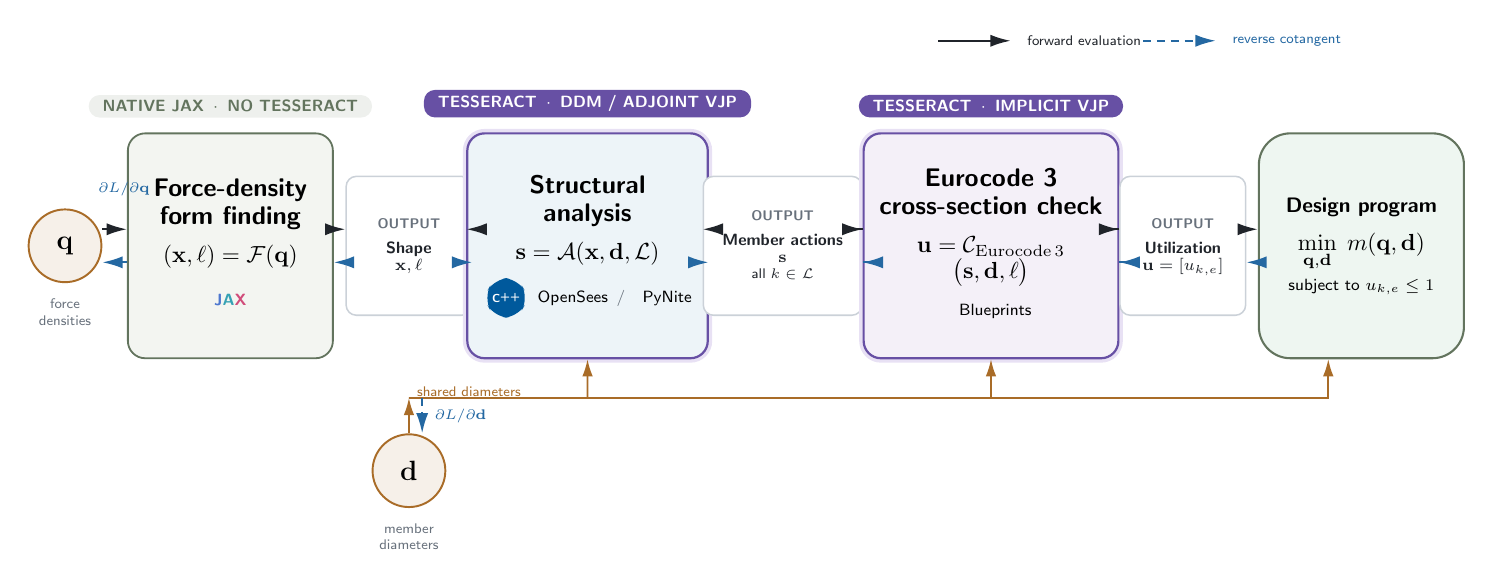
\begin{tikzpicture}[x=1mm,y=1mm,scale=0.84, every node/.style={transform shape}]
  % Primary design variable and the three composed functions.
  \node[design variable] (q) at (0,0) {$\mathbf q$};
  \node[below=1.2mm of q, tiny label, align=center]
    {force\\densities};

  \node[native stage] (form) at (25,0) {\begin{tabular}{@{}c@{}}
    \bfseries\fontsize{10.5}{11.5}\selectfont Force-density\\
    \bfseries\fontsize{10.5}{11.5}\selectfont form finding\\[1.5mm]
    $(\mathbf x,\boldsymbol\ell)=\mathcal F(\mathbf q)$\\[2.3mm]
    \fontsize{7.3}{8}\selectfont \JAXLogo
  \end{tabular}};

  \node[product] (shape) at (52,0) {\begin{tabular}{@{}c@{}}
    \color{Muted}\bfseries\fontsize{6.2}{6.8}\selectfont OUTPUT\\[1mm]
    \color{Ink}\bfseries Shape\\[-0.2mm]
    \color{Ink}$\mathbf x,\boldsymbol\ell$
  \end{tabular}};

  \node[crossed stage] (analysis) at (79,0) {\begin{tabular}{@{}c@{}}
    \bfseries\fontsize{10.5}{11.5}\selectfont Structural\\
    \bfseries\fontsize{10.5}{11.5}\selectfont analysis\\[1.5mm]
    $\mathbf s=\mathcal A(\mathbf x,\mathbf d,\mathcal L)$\\[1.6mm]
    \fontsize{6.8}{7.5}\selectfont
      \CppLogo\enspace OpenSees\enspace\textcolor{Muted}{/}\enspace
      \PythonLogo\enspace PyNite
  \end{tabular}};

  \node[action product] (actions) at (108.5,0) {\begin{tabular}{@{}c@{}}
    \color{Muted}\bfseries\fontsize{6.2}{6.8}\selectfont OUTPUT\\[1mm]
    \color{Ink}\bfseries Member actions\\[-0.3mm]
    \color{Ink}$\mathbf s$\\[-0.4mm]
    \color{Ink}\fontsize{6.5}{7}\selectfont all $k\in\mathcal L$
  \end{tabular}};

  \node[check stage] (check) at (140,0) {\begin{tabular}{@{}c@{}}
    \bfseries\fontsize{10.5}{11.5}\selectfont Eurocode 3\\
    \bfseries\fontsize{10.5}{11.5}\selectfont cross-section check\\[1.5mm]
    $\mathbf u=\mathcal C_{\mathrm{Eurocode\,3}}$\\[-0.4mm]
    $\bigl(\mathbf s,\mathbf d,\boldsymbol\ell\bigr)$\\[1.5mm]
    \fontsize{7}{7.6}\selectfont \PythonLogo\enspace Blueprints
  \end{tabular}};

  \node[product] (utilization) at (169,0) {\begin{tabular}{@{}c@{}}
    \color{Muted}\bfseries\fontsize{6.2}{6.8}\selectfont OUTPUT\\[1mm]
    \color{Ink}\bfseries Utilization\\[-0.2mm]
    \color{Ink}$\mathbf u=[u_{k,e}]$
  \end{tabular}};

  \node[terminal] (program) at (196,0) {\begin{tabular}{@{}c@{}}
    \bfseries\fontsize{9.2}{10}\selectfont Design program\\[1.5mm]
    $\displaystyle\min_{\mathbf q,\mathbf d}\;m(\mathbf q,\mathbf d)$\\[0.7mm]
    \fontsize{7.2}{8}\selectfont subject to $u_{k,e}\leq 1$
  \end{tabular}};

  % Differentiation strategy: explicit labels make the Tesseract boundary
  % visible without enclosing half the figure in a decorative container.
  \node[native badge, above=2.2mm of form]
    {NATIVE JAX \,$\boldsymbol\cdot$\, NO TESSERACT};
  \node[tess badge, above=2.2mm of analysis]
    {TESSERACT \,$\boldsymbol\cdot$\, DDM / ADJOINT VJP};
  \node[tess badge, above=2.2mm of check]
    {TESSERACT \,$\boldsymbol\cdot$\, IMPLICIT VJP};

  % Parallel lanes: primal values move right, output cotangents move left.
  \foreach \left/\right in {q/form,form/shape,shape/analysis,%
    analysis/actions,actions/check,check/utilization,utilization/program}{
    \draw[forward]
      ([yshift=2.5mm]\left.east) -- ([yshift=2.5mm]\right.west);
    \draw[reverse]
      ([yshift=-2.5mm]\right.west) -- ([yshift=-2.5mm]\left.east);
  }

  % Section sizes are shared by analysis, checking, and the mass objective.
  % Their forward and reverse routes sit below the main composition so the
  % central message remains readable at journal-column scale.
  \node[design variable] (d) at (52,-34) {$\mathbf d$};
  \node[below=1.2mm of d, tiny label, align=center]
    {member\\diameters};
  \coordinate (dbus) at (52,-23);
  \draw[parameter feed] (d.north) -- (dbus);
  \draw[draw=Parameter,line width=0.62pt]
    (dbus) -- (140,-23);
  \draw[parameter feed] (79,-23) -- (analysis.south);
  \draw[parameter feed] (140,-23) -- (check.south);
  \draw[parameter feed]
    (140,-23) -| ([xshift=-5mm]program.south);
  \draw[reverse]
    ([xshift=2.0mm]dbus) -- ([xshift=2.0mm]d.north)
    node[midway,right=0.6mm,tiny label,text=Reverse] {$\partial L/\partial\mathbf d$};
  \node[tiny label,text=Parameter,above=0.9mm of dbus,anchor=west]
    {shared diameters};

  % Compact legend, aligned with the figure's optical top edge.
  \draw[forward] (132,31) -- (143,31)
    node[right=1.2mm,tiny label,text=Ink] {forward evaluation};
  \draw[reverse] (163,31) -- (174,31)
    node[right=1.2mm,tiny label,text=Reverse] {reverse cotangent};

  % The final reverse arrow is named once: all local cotangents accumulate in
  % the gradient seen by the constrained optimizer.
  \node[tiny label,text=Reverse,above=0.7mm of q,anchor=south west,xshift=3.8mm]
    {$\partial L/\partial\mathbf q$};
\end{tikzpicture}
\end{document}
